\documentclass{article}

\usepackage{graphicx}
\usepackage{subfigure}
\usepackage[hypcap]{caption}
\usepackage{listings}
\usepackage{float}
\floatstyle{plaintop}
\restylefloat{table}

\title{Experimental Design and Data Analysis: Assignment 4}
\author{Andrew Bedard(2566978) \& Simone van Gompel(2567525) \\ Group 19}

\begin{document}

  \maketitle

  \section*{Exercise 1}
    \subsection*{1}
      \begin{lstlisting}[language=R]
      sample_slices = sample(1:18, 18)
      \end{lstlisting}
    
    \subsection*{2}
      \begin{figure}[H]
          \centering
          \subfigure[Humidity]
          {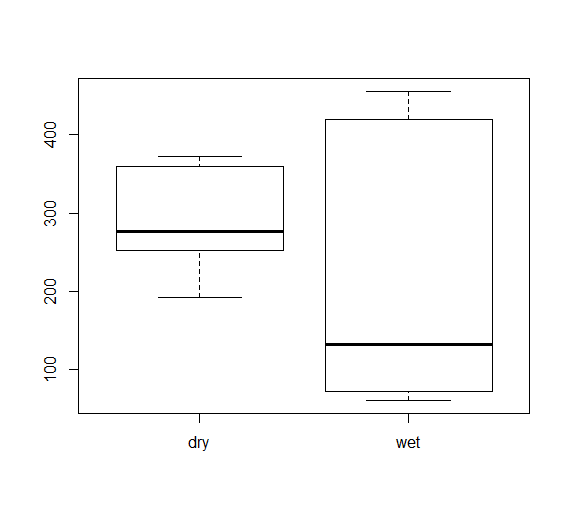
\includegraphics[scale=0.2]{../results/BoxHoursHum.png} }
          \subfigure[Environment]
          {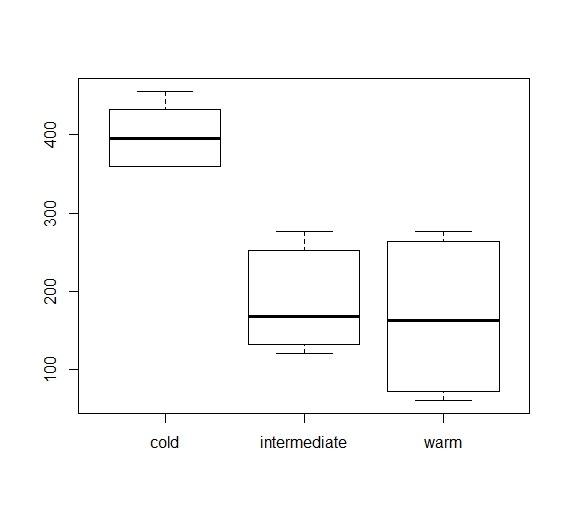
\includegraphics[scale=0.2]{../results/BoxHoursEnv.png} }
          \caption{Boxplots of Hours with Humidity and Environment}
          \label{fig:BoxHours}
      \end{figure} 
    
    \subsection*{3}
      \begin{figure}[H]
          \centering
          \subfigure[Humidity]
          {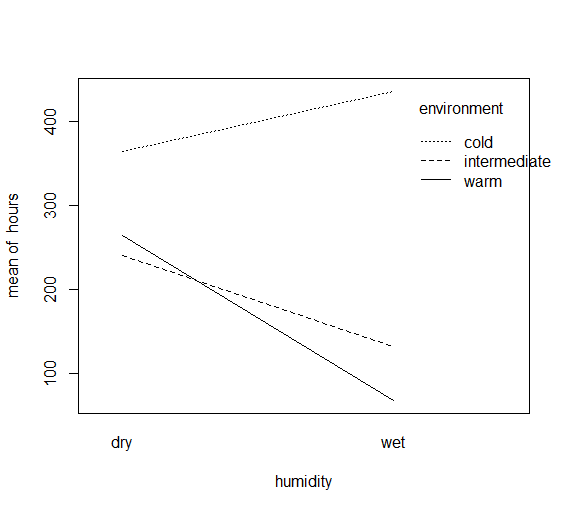
\includegraphics[scale=0.2]{../results/IntPlotHoursHum.png} }
          \subfigure[Environment]
          {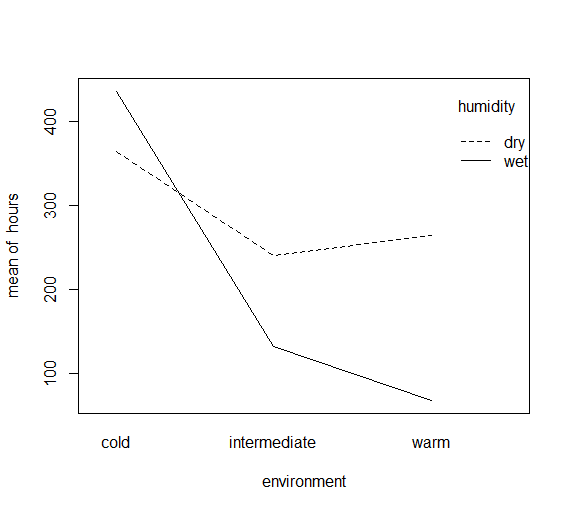
\includegraphics[scale=0.2]{../results/IntPlotHoursEnv.png} }
          \caption{Interactionplots of Hours with Humidity and Environment}
          \label{fig:IntPlotHours}
      \end{figure}
    
    \subsection*{4}
      Analysis of variance on both factors:\\\\
      \begin{lstlisting}[language=R]
Analysis of Variance Table

Response: hours
            Df Sum Sq Mean Sq F value    Pr(>F)    
environment  2 201904  100952 23.1057 3.674e-05 ***
humidity     1  26912   26912  6.1596   0.02637 *  
Residuals   14  61168    4369                      
---
Signif. codes:  0 ‘***’ 0.001 ‘**’ 0.01 ‘*’ 0.05 ‘.’ 0.1 ‘ ’ 1
      \end{lstlisting}
    
    \subsection*{5}
    
    \subsection*{6}
    
    \subsection*{7}
    
    \subsection*{8}
    
  \section*{Exercise 2}
    \subsection*{1}
     
    \subsection*{2}
    
    \subsection*{3}
    
    \subsection*{4}
    
    \subsection*{5}
    
    \subsection*{6}
    
    \subsection*{7}
    
  \section*{Exercise 3}
    \subsection*{1}
      \begin{lstlisting}[language=R]
Analysis of Variance Table

Response: acidity
          Df Sum Sq Mean Sq F value   Pr(>F)   
starter    4 44.136 11.0340  8.0835 0.001106 **
batch      1  4.855  4.8547  3.5566 0.078826 . 
position   4  2.348  0.5870  0.4300 0.784786   
Residuals 15 20.475  1.3650                    
---
Signif. codes:  0 ‘***’ 0.001 ‘**’ 0.01 ‘*’ 0.05 ‘.’ 0.1 ‘ ’ 1
      \end{lstlisting}
    
    \subsection*{2}
      \begin{lstlisting}[language=R]
Call:
lm(formula = acidity ~ starter + batch + position, data = cream)

Residuals:
    Min      1Q  Median      3Q     Max 
-1.7512 -0.7596  0.0132  0.8816  1.0856 

Coefficients:
            Estimate Std. Error t value Pr(>|t|)    
(Intercept)   7.8260     0.8586   9.115 1.67e-07 ***
starter2     -0.1500     0.7389  -0.203  0.84186    
starter3     -0.9800     0.7389  -1.326  0.20459    
starter4      2.8100     0.7389   3.803  0.00173 ** 
starter5     -0.4840     0.7389  -0.655  0.52238    
batch         0.3116     0.1652   1.886  0.07883 .  
position2    -0.6180     0.7389  -0.836  0.41608    
position3    -0.0380     0.7389  -0.051  0.95966    
position4    -0.7640     0.7389  -1.034  0.31755    
position5    -0.2640     0.7389  -0.357  0.72586    
---
Signif. codes:  0 ‘***’ 0.001 ‘**’ 0.01 ‘*’ 0.05 ‘.’ 0.1 ‘ ’ 1

Residual standard error: 1.168 on 15 degrees of freedom
Multiple R-squared:  0.7149,  Adjusted R-squared:  0.5438 
F-statistic: 4.179 on 9 and 15 DF,  p-value: 0.007304
      \end{lstlisting}
    
    \subsection*{3}
      \begin{lstlisting}[language=R]
Linear Hypotheses:
           Estimate Std. Error t value Pr(>|t|)    
2 - 1 == 0  -0.1500     0.4673  -0.321    0.997    
3 - 1 == 0  -0.9800     0.4673  -2.097    0.282    
4 - 1 == 0   2.8100     0.4673   6.013   <0.001 ***
5 - 1 == 0  -0.4840     0.4673  -1.036    0.834    
3 - 2 == 0  -0.8300     0.4673  -1.776    0.429    
4 - 2 == 0   2.9600     0.4673   6.334   <0.001 ***
5 - 2 == 0  -0.3340     0.4673  -0.715    0.949    
4 - 3 == 0   3.7900     0.4673   8.110   <0.001 ***
5 - 3 == 0   0.4960     0.4673   1.061    0.822    
5 - 4 == 0  -3.2940     0.4673  -7.048   <0.001 ***
      \end{lstlisting}
    
    \subsection*{4}
    
    \subsection*{5}
      \begin{lstlisting}[language=R]
Linear Hypotheses:
           Estimate lwr     upr    
2 - 1 == 0 -0.1500  -1.6391  1.3391
3 - 1 == 0 -0.9800  -2.4691  0.5091
4 - 1 == 0  2.8100   1.3209  4.2991
5 - 1 == 0 -0.4840  -1.9731  1.0051
3 - 2 == 0 -0.8300  -2.3191  0.6591
4 - 2 == 0  2.9600   1.4709  4.4491
5 - 2 == 0 -0.3340  -1.8231  1.1551
4 - 3 == 0  3.7900   2.3009  5.2791
5 - 3 == 0  0.4960  -0.9931  1.9851
5 - 4 == 0 -3.2940  -4.7831 -1.8049
      \end{lstlisting}
    
  \section*{Exercise 4}
    \subsection*{1}
    
    \subsection*{2}
    
    \subsection*{3}
    
    \subsection*{4}

    
  \section{R-Code}
    \subsection{Exercise 1}\label{sec:RE1}
      \begin{lstlisting}[language=R]
      \end{lstlisting}
    \subsection{Exercise 2}\label{sec:RE2}
      \begin{lstlisting}[language=R]
      \end{lstlisting}
    \subsection{Exercise 3}\label{sec:RE3}
      \begin{lstlisting}[language=R]
      \end{lstlisting}
    \subsection{Exercise 4}\label{sec:RE4}
      \begin{lstlisting}[language=R]
      \end{lstlisting}
\end{document}
